% =====================================================================
% Primera parte – 6. Modelo de diseño
% =====================================================================
\section{Modelo de diseño del sistema}

Todos los diagramas de esta sección son \textbf{de implementación}: sus clases, atributos, métodos y relaciones son los del código de la rama \codigo{fix/defectos}, después de la refactorización que separó la capa de servicios. La notación sigue UML 2.5.1 \parencite{omg2017}. El modelo conceptual de la entrega anterior se reemplaza por estos diagramas, que lo cubren y además coinciden con el código.

\tikzset{
  clase/.style={draw, rectangle split, rectangle split parts=2, rectangle split part align={center,left},
                font=\scriptsize, inner sep=2.5pt, fill=white},
  clase3/.style={clase, rectangle split parts=3, rectangle split part align={center,left,left}},
  composicion/.style={{Diamond[open=false, length=3mm, width=2mm]}-, thin},
  asociacion/.style={-{Stealth[length=2mm]}, thin},
  usa/.style={-{Stealth[length=2mm]}, thin, dashed, gris},
  mult/.style={font=\tiny, inner sep=1pt},
}

\subsection{Diagrama de clases de implementación}\label{sec:clases-impl}

El backend se organiza en cuatro capas: \textbf{entidades} (\codigo{models.py}, SQLAlchemy), \textbf{validación} (\codigo{schemas.py}, Pydantic), \textbf{servicios} (\codigo{services/}) y \textbf{presentación de la API} (\codigo{routes/}). La Figura \ref{fig:clases-entidades} muestra las entidades persistentes y la Figura \ref{fig:clases-servicios}, los servicios y las rutas que las usan.

\begin{figure}[H]
\centering
\caption{Diagrama de clases de las entidades (\codigo{models.py})}
\label{fig:clases-entidades}
\resizebox{\linewidth}{!}{%
\begin{tikzpicture}
\node[clase, text width=5.2cm, anchor=north] (user) at (0,0) {\textbf{User}
  \nodepart{second}
  + user\_id: int \{PK\}\\
  + username: String(25)\\
  + email: String(150) \{único\}\\
  + password: String(255) \{hash bcrypt\}\\
  + profile\_pic: String(150) [0..1]\\
  + currency: String(10) = "COP"\\
  + created\_at: TIMESTAMP};
\node[clase, text width=5.6cm, anchor=north] (goal) at (-7.4,0) {\textbf{SavingGoal}
  \nodepart{second}
  + goal\_id: int \{PK\}\\
  + user\_id: int \{FK\}\\
  + name: String(100)\\
  + target\_amount: Numeric(15,2)\\
  + start\_date: Date\\
  + end\_date: Date [0..1]\\
  + image\_url: Text [0..1]\\
  + completed\_days: JSON (list[int])\\
  + daily\_amounts: JSON (dict[str, float])\\
  + created\_at: TIMESTAMP};
\node[clase, text width=5.8cm, anchor=north] (cat) at (7.4,0) {\textbf{Category}
  \nodepart{second}
  + category\_id: int \{PK\}\\
  + user\_id: int \{FK\} [0..1]\\
  + name\_cat: String(25)\\
  + icon: String(150) [0..1]\\
  + type: String(10) \{expense, income, both\}\\
  + is\_default: SmallInteger};
\node[clase, text width=5.8cm, anchor=north] (tr) at (-3.4,-6.4) {\textbf{Transaction}
  \nodepart{second}
  + trans\_id: int \{PK\}\\
  + user\_id: int \{FK\}\\
  + category\_id: int \{FK, RESTRICT\}\\
  + type: String(15) \{expense, income\}\\
  + amount: Numeric(15,2)\\
  + description: String(250) [0..1]\\
  + trans\_date: Date = CURRENT\_DATE\\
  + is\_recurring: Boolean = False\\
  + frequency: String(15) [0..1]};
\node[clase, text width=5.8cm, anchor=north] (bud) at (5.2,-6.4) {\textbf{Budget}
  \nodepart{second}
  + budget\_id: int \{PK\}\\
  + user\_id: int \{FK\}\\
  + category\_id: int \{FK, CASCADE\}\\
  + name: String(100)\\
  + amount: Numeric(15,2)\\
  + period\_type: String(10)\\
  + month, year: SmallInteger [0..1]\\
  + start\_date, end\_date: Date [0..1]\\
  + is\_permanent: Boolean = False};
\node[draw, font=\scriptsize, fill=grisclaro] (base) at (0,1.1) {Todas las clases heredan de «SQLAlchemy» Base (\texttt{database.Base})};
% Composiciones desde User
\draw[composicion] ([yshift=-8mm]user.north west) -- node[mult, above, pos=0.15]{1} node[mult, above, pos=0.85]{0..*} node[mult, below, pos=0.5]{saving\_goals} ([yshift=-8mm]user.north west -| goal.east);
\draw[composicion] ([yshift=-8mm]user.north east) -- node[mult, above, pos=0.15]{0..1} node[mult, above, pos=0.85]{0..*} node[mult, below, pos=0.5]{categories} ([yshift=-8mm]user.north east -| cat.west);
\draw[composicion] ([xshift=-12mm]user.south) -- node[mult, left, pos=0.15]{1} node[mult, left, pos=0.85]{0..*} node[mult, left, pos=0.5]{transactions} ([xshift=-12mm]user.south |- tr.north);
\draw[composicion] ([xshift=12mm]user.south) -- node[mult, right, pos=0.15]{1} node[mult, right, pos=0.85]{0..*} node[mult, right, pos=0.5]{budgets} ([xshift=12mm]user.south |- bud.north);
% Category con Budget (composición) y Transaction (asociación)
\draw[composicion] ([xshift=10mm]cat.south) -- node[mult, right, pos=0.1]{1} node[mult, right, pos=0.9]{0..*} node[mult, right, pos=0.5]{budgets} ([xshift=10mm]cat.south |- bud.north);
\draw[asociacion] ([yshift=-6mm]tr.north east) -- node[mult, above, pos=0.06]{0..*} node[mult, above, pos=0.95]{1} node[mult, above, pos=0.6, sloped]{category} ([xshift=-12mm]cat.south);
\end{tikzpicture}}
\figurenote{El rombo relleno indica composición: al eliminar el todo se eliminan las partes (\codigo{cascade="all, delete-orphan"} en el ORM y \codigo{ON DELETE CASCADE} en la BD). La asociación Transaction → Category usa \codigo{ON DELETE RESTRICT}: no se puede borrar una categoría con transacciones (D-05). Fuente: elaboración propia a partir de \codigo{backend/app/models.py}.}
\end{figure}

\begin{landscape}
\begin{figure}[H]
\centering
\caption{Diagrama de clases de servicios, rutas y módulos de soporte}
\label{fig:clases-servicios}
\resizebox{!}{0.72\textheight}{%
\begin{tikzpicture}
% Rutas
\node[clase, anchor=north west, text width=7.0cm] (rb) at (0,0) {\textbf{«router» routes.budgets}\\\codigo{/budgets}
  \nodepart{second}
  + get\_budgets(user, db): list[BudgetOut]\\
  + create\_budget(data, user, db): BudgetOut\\
  + update\_budget(id, data, user, db): BudgetOut\\
  + delete\_budget(id, user, db): None};
\node[clase, anchor=north west, text width=7.6cm] (rs) at (8.2,0) {\textbf{«router» routes.savings}\\\codigo{/saving-goals}
  \nodepart{second}
  + list\_saving\_goals(user, db): list[SavingGoalOut]\\
  + get\_saving\_goal\_detail(id, user, db): SavingGoalOut\\
  + create\_saving\_goal(goal, user, db): SavingGoalOut\\
  + update\_saving\_goal(id, data, user, db): SavingGoalOut\\
  + delete\_saving\_goal(id, user, db): dict\\
  + toggle\_day(id, n, user, db): dict};
\node[clase, anchor=north west, text width=7.6cm] (rt) at (17.0,0) {\textbf{«router» routes.transactions}\\\codigo{/transactions}
  \nodepart{second}
  + get\_categories(user, db): list[CategoryOut]\\
  + create\_transaction(t, user, db): TransactionOut\\
  + get\_transactions(user, db): list[TransactionOut]\\
  + update\_transaction(id, data, user, db): TransactionOut\\
  + delete\_transaction(id, user, db): None\\
  - \_to\_transaction\_out(t): TransactionOut};
\node[clase, anchor=north west, text width=7.6cm] (rc) at (17.0,-15.0) {\textbf{«router» routes.categories}\\\codigo{/categories}
  \nodepart{second}
  + get\_categories(user, db)\\
  + create\_category(data, user, db)\\
  + update\_category(id, data, user, db)\\
  + delete\_category(id, user, db) \{409 si tiene transacciones\}};
\node[clase, anchor=north west, text width=6.6cm] (ru) at (8.2,-15.0) {\textbf{«router» routes.users}\\\codigo{/auth}
  \nodepart{second}
  + register(user, db): UserOut\\
  + login(credentials, db): TokenWithUser\\
  + google\_auth(body, db): TokenWithUser};
\node[clase, anchor=north west, text width=6.0cm] (rp) at (0,-15.0) {\textbf{«router» routes.profile}\\\codigo{/users}
  \nodepart{second}
  + get\_me, update\_me\\
  + update\_password, update\_currency\\
  + upload\_picture, delete\_picture\\
  + delete\_me};
% Servicios
\node[clase, anchor=north west, text width=7.4cm, draw=acento, very thick] (sb) at (0,-6.2) {\textbf{«service» budget\_service}
  \nodepart{second}
  + get\_date\_range(budget, today): tuple[date, date]\\
  + calculate\_spent(db, budget): float\\
  + percentage\_used(spent, amount): float\\
  + to\_budget\_out(db, budget): BudgetOut\\
  + get\_owned\_budget(db, user\_id, budget\_id): Budget\\
  + create\_budget(db, user\_id, data): Budget\\
  + update\_budget(db, budget, data): Budget\\
  - \_reference\_date, \_daily\_range, \_weekly\_range,\\
  \ \ \_monthly\_range, \_unique\_range};
\node[clase, anchor=north west, text width=8.4cm, draw=acento, very thick] (ss) at (8.2,-6.2) {\textbf{«service» saving\_service}
  \nodepart{second}
  + CURRENCY\_CONFIG: dict; DEFAULT\_DURATION\_DAYS = 30\\
  + get\_min\_unit(currency): float\\
  + round\_to\_unit(value, unit): float\\
  + generate\_daily\_amounts(start, end, target, currency): dict\\
  + calculate\_progress(completed, amounts, target): dict\\
  + goal\_progress(goal): dict\\
  + to\_goal\_out(goal): SavingGoalOut\\
  + get\_owned\_goal(db, user\_id, goal\_id): SavingGoal\\
  + create\_goal(db, user, data): SavingGoal\\
  + update\_goal(db, user, goal, data): SavingGoal\\
  + toggle\_day(db, goal, n): dict\\
  - \_distribute\_insufficient, \_distribute\_variable,\\
  \ \ \_as\_list, \_as\_dict};
\node[clase, anchor=north west, text width=7.6cm, draw=acento, very thick] (sc) at (17.0,-6.2) {\textbf{«service» category\_service}
  \nodepart{second}
  + visible\_to(user\_id): condición SQL\\
  + get\_accessible\_category(db, user\_id, id): Category};
% Soporte
\node[clase, anchor=north west, text width=6.6cm] (au) at (3.0,-19.2) {\textbf{«module» auth}
  \nodepart{second}
  + hash\_password(password): str\\
  + verify\_password(plain, hashed): bool\\
  + create\_access\_token(data): str\\
  + get\_current\_user(token, db): User};
\node[clase, anchor=north west, text width=6.0cm] (sch) at (10.6,-19.2) {\textbf{«module» scheduler}
  \nodepart{second}
  - \_toca\_hoy(t, hoy): bool\\
  + registrar\_recurrentes(): None\\
  + scheduler: BackgroundScheduler};
\node[clase, anchor=north west, text width=5.0cm] (db) at (17.6,-19.2) {\textbf{«module» database}
  \nodepart{second}
  + engine, SessionLocal, Base\\
  + get\_db(): Session};
\node[draw, font=\scriptsize, fill=grisclaro, text width=5cm, align=center, anchor=north west] (mod) at (17.6,-22.2) {models: User, Category, Budget, Transaction, SavingGoal (Figura \ref{fig:clases-entidades})\\ schemas: Tabla \ref{tab:schemas}};
% Dependencias
\draw[usa] (rb.south) -- (rb.south |- sb.north);
\draw[usa] (rs.south) -- (rs.south |- ss.north);
\draw[usa] (rt.south) -- (rt.south |- sc.north);
\draw[usa] ([xshift=-6mm]sb.north east) -- ++(0,0.45) -| ([xshift=-14mm]sc.north);
\draw[usa] (rc.north) -- (rc.north |- sc.south);
\draw[usa] (ru.south) -- (ru.south |- au.north);
\draw[usa] (rp.south) -- (rp.south |- au.north);
\draw[usa] (sch.east) -- (sch.east -| db.west);
\end{tikzpicture}}
\figurenote{Las flechas punteadas son dependencias «use». Todas las rutas dependen además de \codigo{auth.get_current_user} y \codigo{database.get_db} por inyección de dependencias de FastAPI (no se dibujan para no saturar). Los servicios con borde de color concentran las reglas de negocio. Fuente: elaboración propia a partir de \codigo{backend/app}.}
\end{figure}
\end{landscape}

\begin{table}[H]
\caption{Esquemas Pydantic (\codigo{schemas.py}) y sus validaciones}
\label{tab:schemas}
\footnotesize
\begin{tabularx}{\linewidth}{L{3.3cm} L{5.3cm} Y}
\toprule
Clase & Atributos & Validaciones \\
\midrule
UserCreate & username, email: EmailStr, password & contraseña $\geq 8$ caracteres \\
UserLogin, UserOut, TokenWithUser, GoogleAuthRequest & email, password; user\_id, username, currency, profile\_pic; access\_token, token\_type, user & formato de correo \\
UserUpdate, PasswordUpdate, CurrencyUpdate & username, email; current\_password, new\_password; currency & nueva contraseña $\geq 8$ \\
CategoryCreate, CategoryUpdate, CategoryOut & name\_cat, icon, type, is\_default & tipo en \{expense, income, both\}; nombre no vacío \\
TransactionCreate, TransactionOut & category\_id, type, amount, description, trans\_date, is\_recurring, frequency; trans\_id, category\_name & monto en (0; 9\,999\,999\,999\,999,99]; tipo en \{expense, income\} \\
BudgetBase, BudgetCreate, BudgetUpdate, BudgetOut & category\_id, name, amount, period\_type, month, year, start\_date, end\_date, is\_permanent; budget\_id, spent, percentage & monto; período válido; mes 1–12; año 2000–2100; período único con fechas ordenadas \\
SavingGoalCreate, SavingGoalUpdate, SavingGoalOut & name, target\_amount, start\_date, end\_date, image\_url; completed\_days, daily\_amounts, progress & monto; nombre no vacío; fin $\geq$ hoy; inicio $\leq$ fin \\
\bottomrule
\end{tabularx}
\tablenote{Los esquemas \codigo{*Out} definen la respuesta; los demás validan la entrada y producen un 422 si fallan. Fuente: elaboración propia.}
\end{table}

\paragraph{Principios aplicados.} Cada servicio tiene una sola responsabilidad (SRP): \codigo{budget_service} calcula períodos y gasto, \codigo{saving_service} genera planes y progreso, y \codigo{category_service} decide qué categorías puede usar un usuario. Las rutas solo traducen HTTP a llamadas de servicio, por lo que la lógica se prueba sin servidor. \codigo{get_date_range} se abrió a nuevos períodos sin modificarse (OCP): basta registrar una función en el diccionario \codigo{_RANGES}.

\subsection{Diagramas de secuencia}\label{sec:secuencia}

Los diagramas muestran las tres funcionalidades centrales y un flujo de soporte. Cada mensaje es una función o un endpoint que existe en el código; los fragmentos \textbf{alt} muestran los flujos alternos y de error.

% Utilidades para diagramas de secuencia
\newcommand{\vida}[4]{% nombre, x, etiqueta, fondo
  \node[caja, fill=white, font=\scriptsize, text width=2.6cm] (#1) at (#2,0) {#3};
  \draw[gris, dashed] (#1.south) -- (#2,#4);}
\newcommand{\msj}[4]{\draw[flecha] (#1,#3) -- node[above, font=\scriptsize, inner sep=1pt]{#4} (#2,#3);}
\newcommand{\resp}[4]{\draw[flechapunteada] (#1,#3) -- node[above, font=\scriptsize, inner sep=1pt]{#4} (#2,#3);}
\newcommand{\auto}[3]{\draw[flecha] (#1,#2) -- ++(0.45,0) -- ++(0,-0.3) -- node[right, font=\scriptsize, inner sep=1pt, align=left]{#3} ++(-0.45,0);}
\newcommand{\marco}[5]{% x1, y1, x2, y2, etiqueta
  \draw[gris] (#1,#2) rectangle (#3,#4);
  \node[draw, gris, fill=white, anchor=north west, font=\tiny\bfseries, text=black, inner sep=1.5pt] at (#1,#2) {#5};}

\begin{landscape}
\begin{figure}[H]
\centering
\caption{Diagrama de secuencia de CU01: Registrar transacción}
\label{fig:sec-cu01}
\resizebox{\linewidth}{!}{%
\begin{tikzpicture}[x=1.3cm, y=0.72cm]
\def\fondo{-17}
\vida{u}{0}{Usuario}{\fondo}
\vida{m}{2.4}{:ModalTransaccion}{\fondo}
\vida{h}{5}{:useTransaccionForm}{\fondo}
\vida{a}{7.6}{api/transactions}{\fondo}
\vida{r}{10.2}{routes.transactions}{\fondo}
\vida{au}{12.8}{auth}{\fondo}
\vida{c}{15.2}{category\_service}{\fondo}
\vida{d}{17.6}{:Session (BD)}{\fondo}
\msj{0}{2.4}{-1.2}{1: clic «+ Transacción», datos, Guardar}
\msj{2.4}{5}{-2}{2: handleSubmit(e)}
\marco{2.1}{-2.4}{5.4}{-3.6}{alt}
\node[font=\tiny, anchor=west] at (2.2,-2.75) {[monto o categoría vacíos]};
\resp{5}{2.4}{-3.3}{3: setError(mensaje)}
\msj{5}{7.6}{-4.2}{4: crearTransaccion(payload)}
\msj{7.6}{10.2}{-5}{5: POST /transactions/ + JWT}
\msj{10.2}{12.8}{-5.8}{6: get\_current\_user(token, db)}
\resp{12.8}{10.2}{-6.6}{7: User}
\auto{10.2}{-7.2}{8: TransactionCreate(...)\\ (validación Pydantic)}
\msj{10.2}{15.2}{-8.6}{9: get\_accessible\_category(db, user\_id, category\_id)}
\msj{15.2}{17.6}{-9.4}{10: query(Category).filter(visible\_to)}
\resp{17.6}{15.2}{-10.2}{11: Category}
\resp{15.2}{10.2}{-11}{12: Category}
\msj{10.2}{17.6}{-11.8}{13: add(Transaction); commit()}
\resp{10.2}{7.6}{-12.6}{14: 200 TransactionOut}
\resp{7.6}{5}{-13.3}{15: data}
\resp{5}{2.4}{-14}{16: onSuccess()}
\resp{2.4}{0}{-14.7}{17: cierra y recarga resumen}
\marco{7.3}{-15.1}{16.1}{-16.9}{alt}
\node[font=\tiny, anchor=west] at (7.4,-15.45) {[token inválido] 6 → 401 \quad [esquema inválido] 8 → 422 \quad [categoría ajena o inexistente] 9 → 404};
\resp{10.2}{7.6}{-16.4}{HTTPException (401 / 422 / 404)}
\end{tikzpicture}}
\figurenote{Fuente: elaboración propia.}
\end{figure}
\end{landscape}

\begin{landscape}
\begin{figure}[H]
\centering
\caption{Diagrama de secuencia de CU02: Gestionar presupuesto}
\label{fig:sec-cu02}
\resizebox{\linewidth}{!}{%
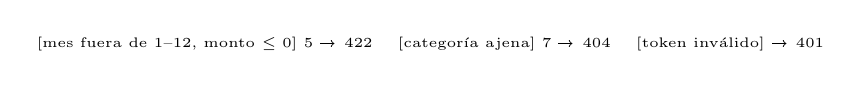
\begin{tikzpicture}[x=1.3cm, y=0.72cm]
\def\fondo{-17}
\vida{u}{0}{Usuario}{\fondo}
\vida{m}{2.4}{:PresupuestoModal}{\fondo}
\vida{h}{5}{:useBudgets}{\fondo}
\vida{a}{7.4}{api/budgets}{\fondo}
\vida{r}{9.8}{routes.budgets}{\fondo}
\vida{s}{12.6}{budget\_service}{\fondo}
\vida{c}{15.2}{category\_service}{\fondo}
\vida{d}{17.6}{:Session (BD)}{\fondo}
\msj{0}{2.4}{-1.2}{1: categoría, nombre, monto, período}
\msj{2.4}{5}{-2}{2: guardar(formData)}
\msj{5}{7.4}{-2.8}{3: crearBudget(data)}
\msj{7.4}{9.8}{-3.6}{4: POST /budgets/ + JWT}
\auto{9.8}{-4.2}{5: BudgetCreate(...)\\(mes, año, período)}
\msj{9.8}{12.6}{-5.6}{6: create\_budget(db, user\_id, data)}
\msj{12.6}{15.2}{-6.4}{7: get\_accessible\_category(...)}
\resp{15.2}{12.6}{-7.2}{8: Category}
\msj{12.6}{17.6}{-8}{9: add(Budget); commit()}
\resp{12.6}{9.8}{-8.8}{10: Budget}
\msj{9.8}{12.6}{-9.6}{11: to\_budget\_out(db, budget)}
\auto{12.6}{-10.2}{12: calculate\_spent(db, budget)\\ \ \ get\_date\_range(budget)}
\msj{12.6}{17.6}{-11.6}{13: query(amount) en categoría y rango}
\resp{17.6}{12.6}{-12.4}{14: montos}
\auto{12.6}{-12.9}{15: percentage\_used(spent, amount)}
\resp{12.6}{9.8}{-14}{16: BudgetOut}
\resp{9.8}{7.4}{-14.6}{17: 201 BudgetOut}
\resp{5}{2.4}{-15.2}{18: lista actualizada}
\resp{2.4}{0}{-15.8}{19: tarjeta (rojo si percentage > 100)}
\marco{7.1}{-16.1}{16.2}{-16.95}{alt}
\node[font=\tiny, anchor=west] at (7.9,-16.5) {[mes fuera de 1–12, monto $\leq 0$] 5 → 422 \quad [categoría ajena] 7 → 404 \quad [token inválido] → 401};
\end{tikzpicture}}
\figurenote{\codigo{get_date_range} elige la función del período (\codigo{_daily_range}, \codigo{_weekly_range}, \codigo{_monthly_range} o \codigo{_unique_range}) y el porcentaje no se limita a 100 (D-04). Fuente: elaboración propia.}
\end{figure}
\end{landscape}

\begin{landscape}
\begin{figure}[H]
\centering
\caption{Diagrama de secuencia de CU03 y CU13: Gestionar meta y marcar días}
\label{fig:sec-cu03}
\resizebox{\linewidth}{!}{%
\begin{tikzpicture}[x=1.3cm, y=0.72cm]
\def\fondo{-20}
\vida{u}{0}{Usuario}{\fondo}
\vida{m}{2.5}{:MetaFormModal /\\VistaMetas}{\fondo}
\vida{h}{5.2}{:useMetaForm /\\useMetas}{\fondo}
\vida{a}{7.6}{api/savings}{\fondo}
\vida{r}{10}{routes.savings}{\fondo}
\vida{s}{13}{saving\_service}{\fondo}
\vida{d}{16.4}{:Session (BD)}{\fondo}
\msj{0}{2.5}{-1.4}{1: nombre, objetivo, fechas}
\msj{2.5}{5.2}{-2.2}{2: handleSubmit(e)}
\msj{5.2}{7.6}{-3}{3: createSavingGoal(payload)}
\msj{7.6}{10}{-3.8}{4: POST /saving-goals/ + JWT}
\auto{10}{-4.4}{5: SavingGoalCreate(...)}
\msj{10}{13}{-5.4}{6: create\_goal(db, user, data)}
\auto{13}{-6}{7: generate\_daily\_amounts(start, end,\\ \ \ target, user.currency)}
\msj{13}{16.4}{-7.6}{8: add(SavingGoal); commit()}
\msj{10}{13}{-8.4}{9: to\_goal\_out(goal)}
\resp{13}{10}{-9.2}{10: SavingGoalOut (progress)}
\resp{10}{7.6}{-9.9}{11: 200 SavingGoalOut}
\resp{2.5}{0}{-10.6}{12: tarjeta de la meta}
\marco{-0.3}{-11.1}{17}{-17.6}{loop [por cada día marcado o desmarcado] (CU13)}
\msj{0}{2.5}{-12.1}{13: marcar días, «Guardar días»}
\msj{2.5}{5.2}{-12.9}{14: alternarDia(goal\_id, n)}
\msj{5.2}{7.6}{-13.6}{15: toggleDay(goal\_id, n)}
\msj{7.6}{10}{-14.3}{16: POST /saving-goals/\{id\}/toggle-day/\{n\}}
\msj{10}{13}{-15}{17: get\_owned\_goal(db, user\_id, id)}
\msj{10}{13}{-15.7}{18: toggle\_day(db, goal, n)}
\msj{13}{16.4}{-16.4}{19: UPDATE completed\_days}
\resp{13}{7.6}{-17.1}{20: \{action, completed\_days, progress\}}
\resp{2.5}{0}{-18.2}{21: «Guardado» y nuevo porcentaje}
\marco{7.3}{-18.6}{16.8}{-19.8}{alt}
\node[font=\tiny, anchor=west] at (7.9,-19.2) {[objetivo $\leq 0$, fecha pasada] 5 → 422 \quad [meta ajena] 17 → 404 \quad [token inválido] → 401};
\end{tikzpicture}}
\figurenote{Sin fecha final, \codigo{create_goal} usa \codigo{DEFAULT_DURATION_DAYS} (D-07); el plan usa la moneda del usuario (D-08) y nunca tiene cuotas negativas (D-01). Fuente: elaboración propia.}
\end{figure}
\end{landscape}

\begin{landscape}
\begin{figure}[H]
\centering
\caption{Diagrama de secuencia de CU05 y CU14: Iniciar sesión y generar recurrentes}
\label{fig:sec-soporte}
\resizebox{\linewidth}{!}{%
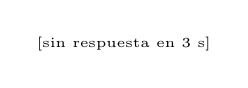
\begin{tikzpicture}[x=1.3cm, y=0.72cm]
\def\fondo{-13.5}
\vida{u}{0}{Usuario}{\fondo}
\vida{p}{2.6}{:AuthPage}{\fondo}
\vida{w}{5.2}{:useBackendWarmup}{\fondo}
\vida{a}{7.8}{api/auth}{\fondo}
\vida{r}{10.4}{routes.users}{\fondo}
\vida{au}{13}{auth}{\fondo}
\vida{sc}{15.6}{scheduler}{\fondo}
\vida{d}{18}{:Session (BD)}{\fondo}
\msj{2.6}{5.2}{-1.2}{1: useBackendWarmup()}
\msj{5.2}{10.4}{-2}{2: GET / (ping)}
\marco{2.3}{-2.4}{6.2}{-3.5}{alt}
\node[font=\tiny, anchor=west] at (2.4,-2.75) {[sin respuesta en 3 s]};
\resp{5.2}{2.6}{-3.2}{3: despertando = true}
\msj{0}{2.6}{-4.2}{4: correo y contraseña}
\msj{2.6}{7.8}{-5}{5: loginUser(email, password)}
\msj{7.8}{10.4}{-5.8}{6: POST /auth/login}
\msj{10.4}{18}{-6.6}{7: query(User).filter(email)}
\msj{10.4}{13}{-7.4}{8: verify\_password(plain, hashed)}
\msj{10.4}{13}{-8.2}{9: create\_access\_token(\{sub\})}
\resp{10.4}{7.8}{-9}{10: 200 TokenWithUser (o 401)}
\resp{2.6}{0}{-9.7}{11: dashboard}
\marco{14.4}{-10.3}{18.6}{-13.3}{loop [cada día 00:05]}
\auto{15.6}{-11.1}{12: registrar\_recurrentes()}
\msj{15.6}{18}{-12.3}{13: \_toca\_hoy(t, hoy) → INSERT si falta}
\end{tikzpicture}}
\figurenote{Fuente: elaboración propia.}
\end{figure}
\end{landscape}

\subsection{Modelo de datos e integridad}

El modelo físico se genera desde \codigo{models.py} con \codigo{Base.metadata.create_all}; sus tablas y columnas son las de la Figura \ref{fig:clases-entidades}. La Tabla \ref{tab:integridad} resume las reglas de borrado tras corregir D-05 y D-11.

\begin{table}[H]
\caption{Restricciones de integridad referencial}
\label{tab:integridad}
\footnotesize
\begin{tabularx}{\linewidth}{L{4.5cm} L{2.4cm} Y}
\toprule
Clave foránea & Al borrar el padre & Comportamiento verificado \\
\midrule
category, budget, transactions, saving\_goal → users & CASCADE & Eliminar la cuenta borra todos sus datos (\codigo{test_pi13_d11_eliminar_cuenta_con_datos_asociados}). \\
budget.category\_id → category & CASCADE & Eliminar una categoría borra sus presupuestos (\codigo{test_pi13_d11_eliminar_categoria_elimina_sus_presupuestos}). \\
transactions.category\_id → category & RESTRICT & Una categoría con transacciones no se borra: 409 (\codigo{test_pi05_d05_*}). \\
\bottomrule
\end{tabularx}
\tablenote{En la base de producción (Supabase) la regla se aplica con la migración \codigo{backend/migraciones/001_transacciones_categoria_restrict.sql}, porque \codigo{create_all} no modifica tablas que ya existen. Fuente: elaboración propia.}
\end{table}

\subsection{Diagrama de componentes}

\begin{figure}[H]
\centering
\caption{Diagrama de componentes y despliegue de ShiftCash}
\label{fig:componentes}
\resizebox{\linewidth}{!}{%
\begin{tikzpicture}[
  comp/.style={caja, fill=white, text width=3.1cm, minimum height=0.9cm},
  nodo/.style={draw, gris, thick, inner sep=8pt},
]
% Frontend
\node[comp] (pages) at (0,0) {«component»\\pages (Home, AuthPage)};
\node[comp] (views) at (0,-2) {«component»\\components: vistas, modales, layout};
\node[comp] (hooks) at (0,-4) {«component»\\hooks (useBudgets, useMetas, useBackendWarmup…)};
\node[comp] (apic) at (0,-6) {«component»\\api/ (Axios + JWT, errores.js)};
\node[comp] (ctx) at (3.8,-2) {«component»\\AuthProvider, PrivateRoute};
\node[comp] (rech) at (3.8,-4) {«library»\\React 19, Router, Recharts};
\node[nodo, fit=(pages)(apic)(ctx)(rech), label={[font=\scriptsize\bfseries]above:«device» Navegador ← Vercel (CDN)}] (fe) {};
% Backend
\node[comp] (routes) at (9.6,0) {«component»\\routes/ (6 routers)};
\node[comp, cajaacento] (serv) at (9.6,-2) {«component»\\services/ (budget, saving, category)};
\node[comp] (sch) at (9.6,-4) {«component»\\schemas.py (Pydantic)};
\node[comp] (mod) at (9.6,-6) {«component»\\models.py + database.py (SQLAlchemy)};
\node[comp] (auth) at (13.4,0) {«component»\\auth.py (JWT, bcrypt)};
\node[comp] (cron) at (13.4,-2) {«component»\\scheduler.py (APScheduler)};
\node[comp] (stat) at (13.4,-4) {«component»\\/static (fotos de perfil)};
\node[nodo, fit=(routes)(mod)(auth)(stat), label={[font=\scriptsize\bfseries]above:«device» Render: Uvicorn + FastAPI}] (be) {};
% Externos
\node[caja, cajagris, text width=3.4cm] (pg) at (9.6,-9.2) {«database»\\PostgreSQL (Supabase)};
\node[caja, cajagris, text width=3.4cm] (goo) at (4.6,-9.2) {«external»\\Google OAuth / userinfo};
\node[caja, cajagris, text width=3.4cm] (gh) at (14.4,-9.2) {«external»\\GitHub Actions (CI y ping)};
% Conexiones
\draw[flecha] (pages) -- (views); \draw[flecha] (views) -- (hooks); \draw[flecha] (hooks) -- (apic);
\draw[flecha] (apic.east) -- node[above, font=\tiny]{HTTPS REST/JSON} (apic.east -| be.west);
\draw[flecha] (routes) -- (serv); \draw[flecha] (serv) -- (sch); \draw[flecha] (sch) -- (mod);
\draw[flecha] (mod.south) -- node[right, font=\tiny]{SQL (psycopg2)} (pg.north);
\draw[flecha] (apic.south) |- node[pos=0.3, left, font=\tiny]{token Google} (goo.west);
\draw[flecha] (be.south -| routes.west) -- node[left, font=\tiny, pos=0.3]{verifica token (/auth/google)} (goo.north east);
\draw[flechapunteada] (gh.north) -- node[right, font=\tiny]{GET /salud cada 10 min} (gh.north |- be.south);
\end{tikzpicture}}
\figurenote{Cada componente es una carpeta o archivo real del repositorio. Fuente: elaboración propia.}
\end{figure}
